%%%%%%%%%%%%%%%%%%%%%%%%%%%%%%%%%%%%%%%%%%%%%%%
\chapter{Decoding FEC Chain} \label{chap:DecodingChain}
%%%%%%%%%%%%%%%%%%%%%%%%%%%%%%%%%%%%%%%%%%%%%%%
In this chapter, implementation and optimization details of 5G polar decoding FEC are presented including challenges faced while achieving low latency decoding. In FEC chain, decoder is the critical part due to inherent sequential nature of polar decoding. $n^{th}$ bit is decoded by using all the previously decoded bits, hence $n^{th}$ bit depends on $0$ to $n-1$ bits. Due to sequential decoding process, significant latency is introduced by the decoder. This section presents the optimization techniques employed to improve decoding FEC chain latency, which include both algorithmic and platform specific optimizations. Each these techniques are explained in the respective sections where these are employed. In this work, FEC chain considered is part of the base station, therefore uplink control information is decoded at receiver. PUCCH (Physical uplink control channel) and PUSCH (Physical uplink shared channel) contain polar encoded information. Received signal after demodulation is quantized to 16-bit LLR (log likelihood ratio) values. Decoding is performed with LLR (Log likelihood ratio) values rather than probabilistic likelihoods due to their numerical stability and low computational complexity. Receiver side FEC chain is a reverse of the operations performed at transmitter. Figure ~\ref{fig:5grx_fec_chain} shows the receiver side polar decoding FEC chain.

\begin{figure}[]
	\centering
	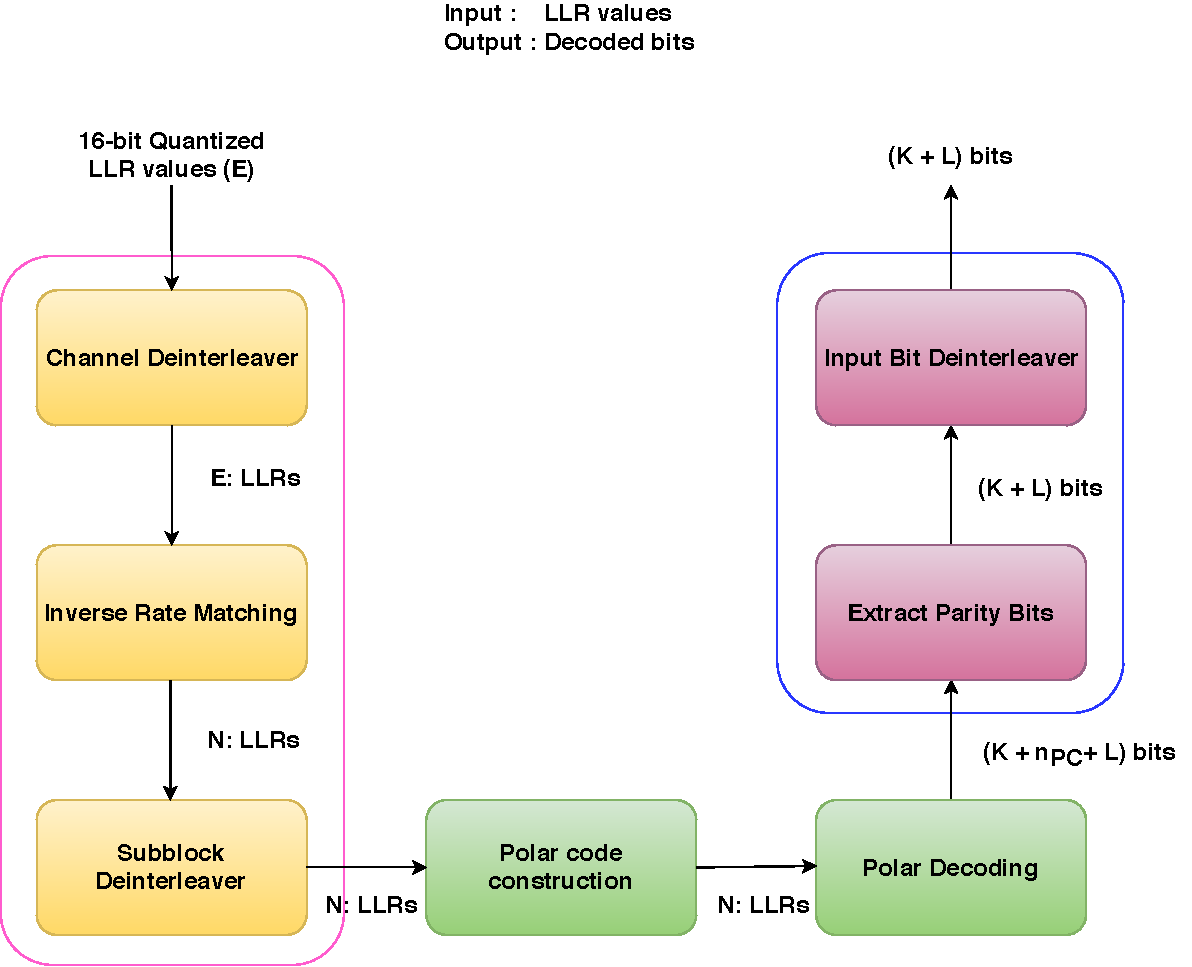
\includegraphics[width=0.82\textwidth]{./figures/receiverFECChain.pdf}
	\caption{Polar decoding FEC chain for PUCCH/PUSCH}
	\label{fig:5grx_fec_chain}
\end{figure}

%$\mathtt{Yadhu}$
%\NOTE{Decoding is of serial nature, has lot of latency. Polar decoding chain necessity. PUCCH and PUSCH, parameters of both the channels.}
%%	Explain all the decoding Optimizations I have done, In this document.
%% 	Explain of the latency without optimization.

\section{Decoding algorithms}
The basic decoding algorithm successive cancellation (SC) is developed by the Arikan in his seminal work on polar codes \cite{Arikan}. It achieves the symmetrical capacity of binary memoryless channel through sequential decoding when block length is very large. However due to the sequential nature significant latency is introduced by decoding algorithm. Latest 5G standard specifies transmission time interval (TTI) of $125 \mu s$ \TODO{cite the doc}, within this duration scheduling and encoding/decoding must be done. Therefore it is very important to efficiently perform FEC chain operations. This work concentrates on implementing the polar encoding/decoding in software and studies the feasibility of satisfying the strict latency requirements of 5G. Decoding through SC algorithm can be represented as binary tree, decoding process is nothing but traversing through a tree sequentially. Significant research work is done both in academia and industry to improve decoding latency of the SC algorithm. Major improvement to SC which significantly reduced the decoding latency is identifying special kind nodes in a tree which allow immediate decoding of multiple bits without requiring full tree traversal. Algorithms presented in \cite{SSC} and \cite{fastSSC} present such improvements, which identify special nodes or in other words component codes such as \textit{Rate-0}, \textit{Rate-1}, \textit{RPC} and \textit{SPC} nodes, \textit{RPC} and \textit{SPC} mean repetition and single parity check code respectively. Identification of special nodes requires finding particular patterns the frozen bit locations in the constructed polar code. To gain full advantages of Fast-SSC (Fast Simplified Successive Cancellation) algorithm, special nodes must be identified efficiently. In this work, 5G RX FEC chain with fast-SSC algorithm implemented/optimized in software and feasibility of achieving desired latency( $< 50\mu s$) is analyzed.
%Following sections present how processor specific features are exploited to efficiently identify


\section{Decoding chain}
The figure ~\ref{fig:5grx_fec_chain} shows the complete receiver side FEC chain. It is almost a inverse operations of encoding FEC chain except few differences related to PUCCH and PDSCH which contain parity check bits ($ n_{PC} $). The decoding FEC chain receives UCI(Uplink Control Information) in the form of 16-bit quantized $ E $ LLR values. Before passing LLR values to decoder inverse operations of the steps which were carried out aftermath of encoding, which are channel deinterleaving, inverse rate matching and subblock deinterleaving. These steps grouped by a pink rectangle in the figure, after these steps polar code construction is performed using same optimized method as presented in the previous chapter. Polar code construction procedure outputs the information bit positions, from which frozen pattern can be obtained. Next step in the FEC chain is polar decoding, $ N $ LLR values and frozen pattern is passed to polar decoder, which outputs the decoded bits. Polar construction and decoding blocks are colored green the FEC chain figure. Using information bit positions obtained in the polar construction procedure $ K + n_{PC} + L $ bits are extracted from $ N $ decoded bits. $ K + n_{PC} + L $ bits contain $ n_{PC} $ parity bits, extracting these bits requires identifying the row of minimum weight from the generator matrix of polar code. Finally input deinterleaving is applied on the remaining $ K +  L $ bits to obtain concatenated information and CRC bits. Blocks representing Extracting parity bits and input bit deinterleaver are grouped with blue rectangle. In this section, we presented briefly the functionalities carried out by different blocks of the decoding FEC chain. Next we will analyze the latency contributions of each those operations and come up with optimizations both algorithmic and platform specific to reduce latency.

\section{Channel deinterlever}
The first operation after receiving the LLR values is channel deinterleaving, This is the exact inverse of the interleaving operation done at the transmitter. Channel interleaving is performed to make transmission robust against burst errors. Authors of \cite{3gpp.TSG-RAN_WG1} analyze the error correction performance of polar codes for different channel conditions and constellations. It is found that error correction performance significantly deteriorates for constellations 16-QAM onwards. Channel interleaving wasn't done for downlink PBCH/PDCCH since the constellation was QPSK, however in case of PUCCH/PUSCH higher constellations are used hence channel interleaving is necessary. In 5G standard  isosceles right triangle interleaver is adopted. Deinterleaving is carried out by writing LLR values to columns of triangular structure and reading LLR values in rows. Interleaver design is proposed by Qualcomm \cite{3gpp.TSG-RAN_WG1}.

Vector processing instructions cannot be used for the implementation of interleaver due irregular and non uniform memory access, therefore interleaver just plain functional implementation. One optimization technique was to avoid new memory allocation and using already allocated memory. This avoids the overhead of dynamic memory allocation and initialization. Channel deinterleaving is one of significant contributor to latency in polar decoding FEC chain, since each of the LLR values need to processed sequentially.

\section{Inverse rate matching}
Inverse rate matching step maps the $E$ LLR values to mother code block size $ N $. Rate matching step has three modes puncturing, shortening and repetition. Mode is selected based on rate matcher output size ($E$) and mother code size($ N $). If $E > N$ then repetition performed, otherwise either puncturing and shortening is done. If $ \frac{K}{E} > \frac{7}{16} $ shortening else puncturing is performed. Major optimization in inverse rate matching are utilizing SIMD capability for soft combining when $ E>N $ and performing block wise copying. \NOTE{Does it makes sense to explain criteria why puncturing or shortening is selected}
%
%to and avoiding a copying operations when the mode is shortening or puncturing instead using a pointer manipulation to select
%Software optimization in inverse rate matching is performed by Empirically it is observed that shi  type of rate matching is selected based on code rate.
%
\section{Sub-block de-interleaver}
After inverse rate matching, $E$ values are mapped to $N$ LLRs, which is always a power of two. Subblock interleaver/deinterlever divides block of $N$ LLRs into $32$ subblocks, each containing $\frac{N}{32}$ LLRs. These subblocks are interleaved as shown in the figure \NOTE{add figure}. Functionally, subblock deinterleaving can be implemented as a inverse operation of algorithm presented in \cite{3gpp.38.212}. Upon measuring the latency contribution of subblock deinterleaver it was found to be taking $10 \mu s$. Computation complexity of interleaving indexes huge due to the use of multiplication, division and modulus operations. \newline


\begin{figure}[]
	\centering
	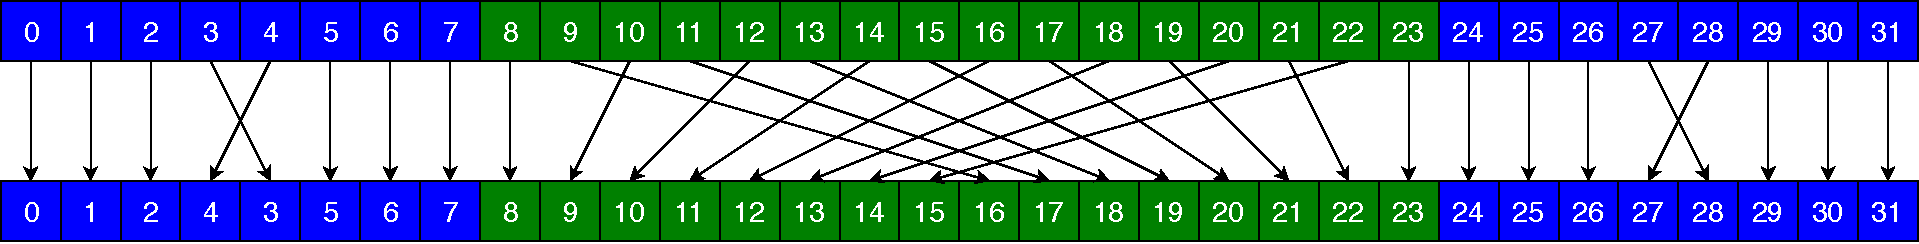
\includegraphics[width=1.0\textwidth]{./figures/subblockDeinterleaver.pdf}
	\caption{Subblock deinterleaving pattern}
	\label{fig:subblockDeinterleaver}
\end{figure}


If we look at the figure ~\ref{fig:subblockDeinterleaver}, we can see that not all the values of LLRs are interleaved, only 18 positions out of 32. Calculating interleaving positions is expensive instead they can be pre-calculated and stored in a lookup table. For the mother code size of 1024, with pre-calculated positions interleaving requires looping for $ 576 $ times. Modern processors with \textit{AVX} and \textit{AVX2} extensions provide special swizzle instructions, which allow shuffling, permuting and blending of vectors. These instructions process vector of values hence allow data parallelism. To make use of swizzle instructions for subblock deinterleaving, it must be reformulated to fit into functionality provided by platform specific SIMD instructions. It is divided into three parts, each one is independent of another. Part one and three are exactly same operations each dealing with 8 subblocks and performing the operation marked by green in the figure. Part two deals with 16 subblocks, marked by blue in the figure. Part two operation is achieved with blend and permute SIMD instructions.

Code snippet in the listing ~\ref{code:subblockDeinterleaver} shows sample SIMD implementation of subblock deinterleaving operation for mother code size ($N$) 64.

\begin{code}
\captionof{listing}{Vectorized Subblock deinterleaving for $N = 64$}
\label{code:subblockDeinterleaver}
\begin{minted}{c++}
void subblockdeinterleaver64( int16_t y[], int16_t d[]) {
	__m256i v256_in,v256_perm0,v256_out,v256_perm1,v256_perm2;
	__m256i v256_out2,v256_blended,v256_perm3;
	//interleaving pattern, precalculated is encoded here.
	v256_perm0 = _mm256_setr_epi32(0,1,2,4,3,5,6,7);
	v256_perm1 = _mm256_setr_epi32(0,2,4,6,1,3,5,7);
	v256_perm2 = _mm256_setr_epi32(1,3,5,7,0,2,4,6);
	v256_perm3 = _mm256_setr_epi32(4,5,6,7,0,1,2,3);
	
	//prepare part1
	v256_in = _mm256_loadu_si256((__m256i*)y);
	v256_out = _mm256_permutevar8x32_epi32 (v256_in,v256_perm0);
	_mm256_storeu_si256((__m256i*)d,v256_out);
	
	//prepare part2
	v256_in = _mm256_loadu_si256((__m256i*)(y + 16));
	v256_out = _mm256_permutevar8x32_epi32 (v256_in,v256_perm1);
	v256_in = _mm256_loadu_si256((__m256i*)(y + 32));
	v256_out2 = _mm256_permutevar8x32_epi32(v256_in,v256_perm2);
	v256_blended = _mm256_blend_epi32 (v256_out,v256_out2,0b11110000);
	_mm256_storeu_si256((__m256i*)(d  + 16),v256_blended);
	v256_out2 = _mm256_permutevar8x32_epi32(v256_out, v256_perm3);
	v256_out = _mm256_permutevar8x32_epi32(v256_in, v256_perm1);
	v256_blended = _mm256_blend_epi32(v256_out2,v256_out,0b11110000);
	_mm256_storeu_si256((__m256i*)(d + 32),v256_blended);
	
	//prepare part3, same as part1
	v256_in = _mm256_loadu_si256((__m256i*)(y + 48));
	v256_out = _mm256_permutevar8x32_epi32 (v256_in,v256_perm0);
	_mm256_storeu_si256((__m256i*)(d + 48),v256_out);	
}
\end{minted}
\end{code}

\begin{code}
\captionof{listing}{Non-vectorized Subblock deinterleaving}
\label{code:slowSubblockDeinterleaver}
\begin{minted}{c}
void subblockdeInterleaver( vector<int16_t> &y, vector<int16_t> &d) const
{
	for (uint32_t n = 0; n < N; n++)
	{
		uint32_t i = floor((n * 32 ) / N);
		uint32_t Jn = P[i] * (N/32) + (n % (N/32));
		d[Jn] = y[n];
	}
}
\end{minted}
\end{code}

Results Latency optimization for subblock deinterleaver $N = 1024$
before 19.7us, after 0.47us 

\section{Decoder optimization}

\subsection{Identifying component codes}
%How different kind of sub code types are identified efficiently using with bit packed frozen bits.
As explained in the beginning of this chapter, naive SC algorithm purely sequential, hence decoder introduces significant latency in the FEC chain. With improvements such as \cite{fastSSC} and \cite{SSC} decoding tree can be pruned by identifying particular patterns in frozen bit positions. Pruning of a tree allows decoding multiple bits in parallel. Component codes out of polar codes can be identified which allow decoding without traversing the full decoder tree. Authors in \cite{SSC} and \cite{fastSSC} identify four such codes namely rate-0, rate-1, repetition and single parity codes. Decoding a code word through component codes improves latency without compromising the error correction performance. However to fully enjoy the fruits decoding tree pruning, implementation should be able identify component codes efficiently. One simple functional way is to go through all frozen bits and search by comparing with predefined patterns. Naive way of searching for a pattern introduces significant latency in the decoding process. Processors with \textit{AVX} and \textit{AVX2} support contain registers which can store 256/128 bits in a single register. Frozen pattern array/vector contain either one or zero, one indicating frozen bit and zero information bit. Since one bit is enough to represent type of bit position, frozen pattern can be stored by packing multiple bits type information to single 256bit register which allows identifying a pattern by comparing with a integer using single SIMD instruction. As an example with a mother code size $N=256$ information about which position is frozen and which is not can stored in a single 256 bit SIMD register in a bit packed format. To check whether it is a rate-0, rate-1, SPC or RPC requires one SIMD comparison instruction. Snippet in a listing ~\ref{code:rateOneSIMDComparison} illustrates an example of identifying node type in bitpacked frozen bits pattern.

\begin{code}
	\captionof{listing}{Check for a rate-1 subcode}
	\label{code:rateOneSIMDComparison}
	\begin{minted}{c++}
template<>
inline int identify_pattern<256>(uint64_t s[],nodeType node) {
	__m256i temp1 = _mm256_loadu_si256 ((__m256i*)s);
	__m256i temp2;
	switch(node) {
	case nodeType::R_0:
		temp2 = _mm256_set1_epi8 ((char)0xFF);
		break;
	case nodeType::R_1:
		temp2 = _mm256_set1_epi8 (0x00);
		break;
	case nodeType::REP:
		temp2 = _mm256_set_epi64x(0xFFFFFFFFFFFFFFFFLL,0xFFFFFFFFFFFFFFFFLL,...
				0xFFFFFFFFFFFFFFFFLL,0xFFFFFFFFFFFFFFFELL);
		break;
	case nodeType::SPC:
		temp2 = _mm256_set_epi64x(0x8000000000000000LL,0x0000000000000000LL,...
				0x0000000000000000LL,0x0000000000000000LL);
		break;
	case nodeType::NO_NODE_TYPES:
		std::cout<<"Invalid node type";
	}
	__m256i pcmp = _mm256_cmpeq_epi64 (temp1, temp2);
	unsigned bitmask = _mm256_movemask_epi8(pcmp);
	return (bitmask == 0xffffffffU);
}
\end{minted}
\end{code}

\subsection{Decoding Rate-0 code}
Rate-0 code is a special kind of node in a decoding tree in which all the descendants represent frozen bit positions, in other words corresponding node's frozen pattern contains all ones. One such example is given in the background section. For such a node, we know that all the bits are frozen hence decoder can immediately decode values as zero. All the decoded bits corresponding to such a node are set to zero. Rate-0 node allows decoder to avoid performing VN and CN operations at the subsequent child nodes in addition to decoding multiple bits simultaneously.

\subsection{Decoding Rate-1 code}
A node is considered as Rate-1 node, if all of its descendants in a decoder tree are information bits. In other words the Rate one node contains no frozen bits. Decoding of Rate-one can also be performed without traversing till the end of a decoder and hence avoiding significant number of VN and CN operation. However decoding Rate-1 node is not as straight forward as Rate-0 node. Decoding is done through threshold detection of all the LLRs and performing polar transform on the result to obtain decoded bits.

\begin{code}
	\captionof{listing}{Decoding rate-1 subcode}
	\label{code:rateOneNodeDecoding}
	\begin{minted}{c++}
template<unsigned Nv>
void decodeR_1_simd(int16_t demodLLRs[],int8_t beta[],int8_t decodedBits[]) {
  eIndex = 0;
  __m128i temp1,tempDecodedVec;
  _m_prefetch(beta);
  _m_prefetch(decodedBits + dIndex);
  for(unsigned i = 0; i < Nv; i = i + 8) {
    temp1 = _mm_loadu_si128((__m128i*)(demodLLRs + i));
    tempDecodedVec = _mm_cmplt_epi16(temp1,zeros);
    tempDecodedVec = tempDecodedVec & _mm_set1_epi16(1);
    tempDecodedVec = _mm_packs_epi16(tempDecodedVec,_mm_setzero_si128());
    _mm_storeu_si128((__m128i*)(beta + i),tempDecodedVec);
    _mm_storeu_si128((__m128i*)(decodedBits + dIndex + i),tempDecodedVec);
  }
  polarTransform<Nv>(decodedBits + dIndex,decodedBits + dIndex);
  dIndex += Nv;
}
\end{minted}
\end{code}

Although Rate-1 nodes avoids CN and VN operations, decoding is not parallel. Decoder needs to go through each of the LLRs to decode the bits and finally perform polar transform both of which are costly operations. To improve the latency through data parallelism, threshold detection can make use of SIMD instructions, which allow threshold detection of a vector through single SIMD comparison instruction.This improves the parallelism factor to sixteen for 16-bit LLRs with {AVX2} instructions. The code snippet in listing ~\ref{code:rateOneNodeDecoding} presents an example where rate-1 node decoding is implemented using AVX instructions resulting in parallelism factor of eight. Next step in decoding rate-1 node is performing polar transform operation. It is equivalent to performing polar encoding. As explained in the previous chapter, binary tree represents encoding process. Efficient polar transform implementation makes use of same optimizations techniques employed in encoder such as SIMD vectorization and look up table techniques.

\subsection{Decoding RPC code}
Repetition code (RPC) is another type of sub code which be identified from polar code. It allows decoding multiple bits without tree full tree traversal. A node is considered as RPC when only one its right most descendent contains information and all remaining bits are frozen. Bit packed frozen pattern allows easy identification of RPC node. If frozen pattern at the node is equal to one then it is a RPC node. RPC node decoding is similar to simple repetition code decoding by adding all the LLRs and doing threshold detection for the sum.  Result of threshold detection is stored at information bit position and remaining bits at the node are set to zero.

\begin{equation*}
 \beta_{v}[i] = \begin{cases}
				0, \text{ when $\sum_{j} \alpha_{v}[j] \geq 0 ;$}  \\
				1, \text{ otherwise.}
				\end{cases}
\end{equation*}

Again, RPC-node decoding process has scope for improvement. Decoding requires summing of all LLRs. Summation operation efficiently performed with SIMD instructions through data parallelism instead of adding individual values. This vectorization has significant gain when sum of huge LLR vector is required.

\subsection{Decoding SPC code}
Another type of constituent codes which can be decoded more efficiently without complete tree traversal is single-parity check (SPC) code. These nodes have a code rate $Nv-1/Nv$. In other words, these nodes have only one frozen bit at right most position. Optimal ML decoding of SPC codes can be performed in an optimal way with very low complexity. Similar to Rate-1 code decoding SPC code requires threshold detection for all the LLRs. To achieve this efficiently same optimizations employed to Rate-1 code are reused. For SPC decoding two more additional steps are required namely finding position of minimum magnitude LLR and calculating the parity of decoded bits. If the parity of decoded bits is not even then bit value at the position of lowest magnitude LLR is flipped. Final step in the decoding is to obtain final decoded bits values through polar transform. The steps described above are shown in the algorithm ~\ref{algo:spcDecoding}.

\IncMargin{1.5em}
\begin{algorithm}[]
	\KwData{$\alpha_{v}^{N_v-1}$, $N_v$}
	\KwResult{$y_{0}^{N_v-1}$, $\beta_{0}^{N_v-1}$}
	\SetKwFunction{FMain}{decodeSpc}
	\SetKwProg{Fn}{function}{:}{}
	\Fn{\FMain{$\alpha_{v}^{N_v-1}$,$y_{0}^{N_v-1}$, $\beta_{0}^{N_v-1}$}} {
			$j = \alpha_{v}[i]$ \;
			$parity = 0$ \;
			\For{$i=0$ to $N_v-1$} {
				$\beta_{v}[i] = \alpha_{v}[i] \ge 0$\;
				\If {$j < |\alpha_{v}[i]|$} {
					$j = i$ \;
				}
				$parity = parity + \beta_{\textit{i}}[i]$ \;
			}
		\If {$parity \neq 0$} {
			$\beta_{v}[j] = 1 - \beta_{v}[j]$\;
		}
		$y_{0}^{N_v-1} = polarTransform(\beta_{0}^{N_v-1})$ \;
		}
	\caption{SPC decoding}
	\label{algo:spcDecoding}
\end{algorithm}
\DecMargin{1.5em}

SPC code uses same two operations (threshold detection and polar transform) as used in RPC decoding. This allows reusing of same optimization techniques. Two additional operations in SPC decoding are finding the position of minimum magnitude LLR and calculating the parity. Time complexity of finding a minimum magnitude LLR position is $\mathcal{O}\big(N\big)$. It can be reduced to $\mathcal{O}\big(N/8\big)$ by mapping search operation to SIMD instruction which processes vectors of size eight in parallel. SSE4.1 instruction $\mathtt{phminposu}$ comes to rescue. It processes vectors of size 128 bits, computes minimum amongst the packed unsigned 16-bit vectors returns the position and its value. Parity calculation of the decoded bits also requires iterating through all bits obtained after threshold detection. Again, to efficiently obtain number of set bits $\mathtt{popcnt}$ instruction is used, which can calculate the number of set bits in a vector. These optimizations reduced the latency of SPC decoding to less than $50\%$ of naive algorithmic implementation shown in ~\ref{algo:spcDecoding}.

\subsection{Partial unrolling of decoder}
Recursive formulation decoders makes it easy to implement in addition to allowing reuse of hardware resources in FPGA/ASIC. Successive cancellation decoding algorithm for polar codes is formulated recursive form. However this formulation has huge disadvantage when it comes to software implementations. Every recursive function call in software requires new stack frame allocation and jump to a starting address of function. Both operations are expensive in terms of processor cycles. Authors in ~\cite{fastPolarDecodersAlgoImpl} propose unrolling of the decoder, hence avoiding recursive function calls and branch instructions. In polar FEC chain of 5G, full unrolling of decoder is not possible due to varying block-length and code rate requirements. Different code rate requirement makes it impossible to know frozen bit positions are compile time, hence it is necessary to dynamically identify presence special nodes in the decoder tree. In this work, partial decoding unrolling is done, i.e recursive function calls are completely avoided. Template concept of C++ language are used for auto unrolling of functions. However still branches are present which check for the presence special nodes in a tree. Partial unrolling also significantly reduced the decoding latency.

\subsection{Cache prefetching}
Performance bottle necks in the modern processors lies in main memory access. To overcome this problem most of modern processors contain smaller fast memory called cache close to the processor. Addition of caches reduces the number of accesses to main memory. However due to the limited cache size it might happen that the requested data not being present in cache, which results in an event called cache-miss. Copied data from main memory to cache has a huge overhead. Cache miss overhead can be reduced by dealing with less memory allocation, in other words reusing the memory as much as possible. Some of the modern processors provide special non blocking instructions which allow cache line prefetching. If the memory access required is known, prefetching instruction can be issued well in advance by software before accessing memory. These instructions if used efficiently, can hide the memory access latency. In this work, decoder implementation is optimized for AMD EPYC platform, which provides cache prefetching instrunctions through $ \mathtt{3dnow} $ extensions. Due to regular memory access in polar decoder, prefetching instructions are used whenever possible to hide memory access latency.

\subsection{Decoder tree pruning}
Decoding latency can be further reduced by minimizing the number of nodes to be traversed in a decoder tree. This is achieved by pruning decoding tree intelligently at a particular level based on the given SNR and code rate. The level of pruning for a particular SNR and code can be determined through simulations. This information can be stored in a look up table which can be used later to determine the level pruning during decoding. Here decoder tree is pruned irrespective frozen pattern type


\section{Extract Info Bits}
Means select information bits from the reliable positions.

\section{Extract parity check bits}

\section{CRC calculation}


